\chapter{Fonctionnement}
\label{chap:fonctionnement}

L'algorithme \aes possède deux modes, le premier est le mode courant GCM et le second est le GMAC.

\section{GCM}

\subsection{Avantanges de GCM}

\aes est un algorithme qui assure un haut niveau de sécurité grâce à AES, mais surtout il assure l'authenticité et l'intégrité des données. C'est à dire que si Alice essaye de communiquer avec Bob, elle est assurée que Charlie ne pourra pas lire ses données mais également qu'il ne pourra pas les modifier sans que Bob s'en aperçoive. 

\begin{figure}[!h]
  \centering
  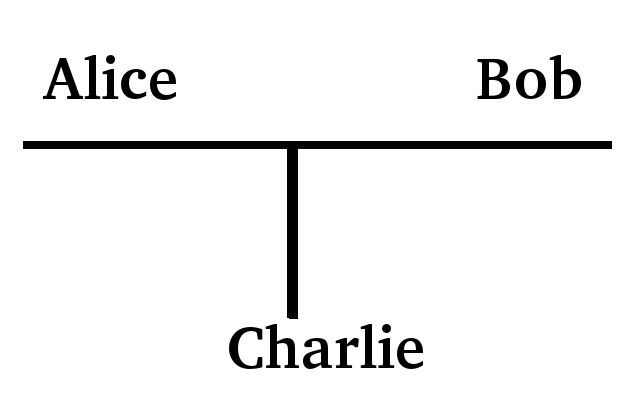
\includegraphics[width=0.5\textwidth]{alice_bob}
  \caption{Bob et Alice}
  \label{Bob et Alice}
\end{figure}

%GCM assure un haut niveau de protection des données. En effet, GCM peut détecter à la fois les modifications de code accidentelles et les modifications non autorisées intentionnelles.

De plus, GCM est un algorithme parallélisable qui assure une implémentation à haut débit à la fois matériel et logiciel.
~\\

Néanmoins, \aes suppose que Alice et Bob se soient au préalable échangés une clef secrète.

\subsection{Acronymes}


Tout d'abord, pour bien expliquer le fonctionnement de \aes, il nous faut définir certains acronymes.

\begin{center}
  \begin{tabular}[h]{|l|l|}
    \hline
    Plaintext&le texte à chiffrer\\
    Ciphertext&le texte chiffré\\
    auth Data&des données supplémentaires à authentifier\\
%    Counter&un élément supposé aléatoire\\
    K&la clé de chiffrement (secret)\\
    H&Sous clé de hachage (secret)\\
    IV& Vecteur d'initialisation supposé aléaoire\\
    Mult&une multiplication dans l'espace de Galois\\
    \hline
  \end{tabular}
\end{center}


\subsection{Chiffrement}

\aes est composé de deux blocs distincts, le bloc de chiffrement et le bloc d'authentification\footnote{On parlera ici d'authenticité lorsque l'on veut s'assurer que le message vient de la bonne personne}-intégrité\footnote{On parlera d'intégrité lorsque l'on veut s'assurer que les données n'ont pas été modifiées}.

Dans un premier temps on va parler du bloc de chiffrement. Dans GCM il y C pour \og counter\fg{}, \cad que \aes s'appuie sur un mode qu'on nomme CTR \footnote{CounTeR}.

Ccomme on peut le voir sur la figure \ref{schema CTR}, ce mode chiffre un compteur avec une clef (K) à travers un algorithme. Ensuite il réalise une opération de type XOR (ou exclusif) sur le texte clair avec la sortie de l'algorithme pour obtenir le texte chiffré.

\begin{figure}[!h]
  \centering
  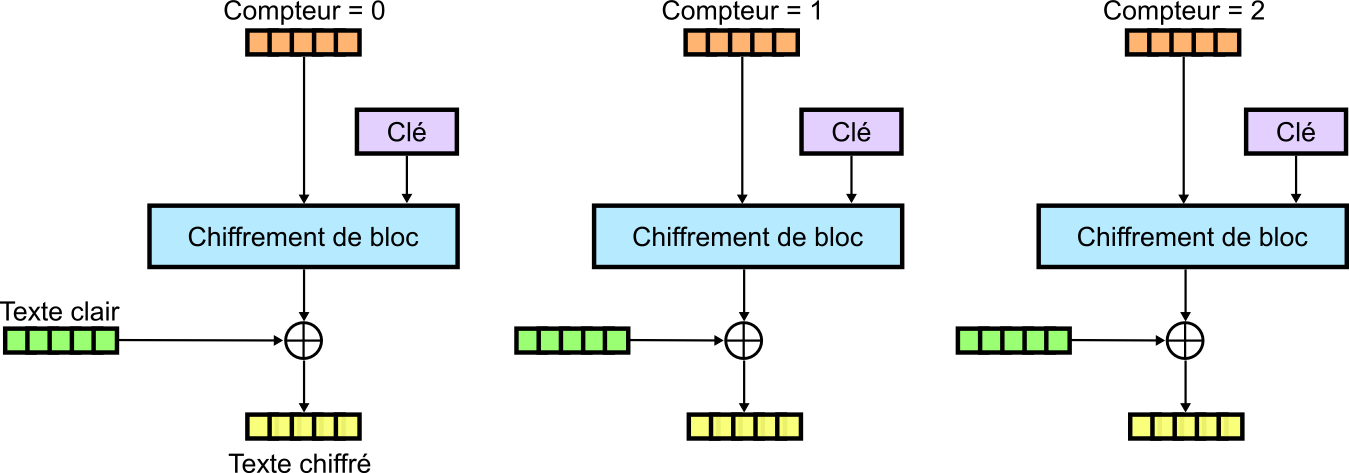
\includegraphics[width=\textwidth]{ctr}
  \caption{schéma CTR \cite{wiki}}
  \label{schema CTR}
\end{figure}

 Ce mode combine les avantages du chiffrement par flots, est pré-calculable et est parallélisable. En effet il est possible de calculer à l'avance en parallèle tous les chiffrés des compteurs. Il ne restera plus qu'à les passer dans la fonction XOR avec le clair pour obtenir le chiffré.
 ~\\

 Dans le cas de \aes le bloc de chiffrement est l'algorithme AES, et le compteur est le vecteur d'initialisation pseudo aléatoire IV qu'on incrémente.


\subsection{Authentification-Intégrité}

L'algorithme GCM permet de créer un Tag qui valide l'authenticité et l'intégrité des données. Pour mieux comprendre nous avons découpé cette opération pour voir tous les éléments qui interviennent dans ce processus.

Tout d'abord, la première chose dont on cherche à s'assurer est l'intégrité des données chiffrées que nous envoyons. En effet, nous avons chiffré notre texte mais rien ne nous protège contre une modification intentionnelle ou accidentelle du message envoyé. Ainsi, si Charlie cherche à gêner la communication de Bob et Alice et qu'il change certains bits on voudrait s'en rendre compte. On pourrait réaliser un hash de notre message avec des fonctions comme sha ou md5, mais si on fait cela on ne pourra pas être protégé contre les modifications intentionnelles. Charlie n'aurait qu'à remplacer le hash par le hash du message contenant sa modification. La solution retenue dans GCM est d'utiliser des multiplications dans l'espace de Galois avec une autre clef nommée H secrète. On fait donc passer le premier bloc de chiffrés dans un bloc de multiplication avec H. Puis on réalise un XOR du résultat avec le bloc de chiffré suivant. Enfin on refait la multiplication comme on peut le voir sur l'image \ref{auth1}.

\begin{figure}[!h]
  \centering
  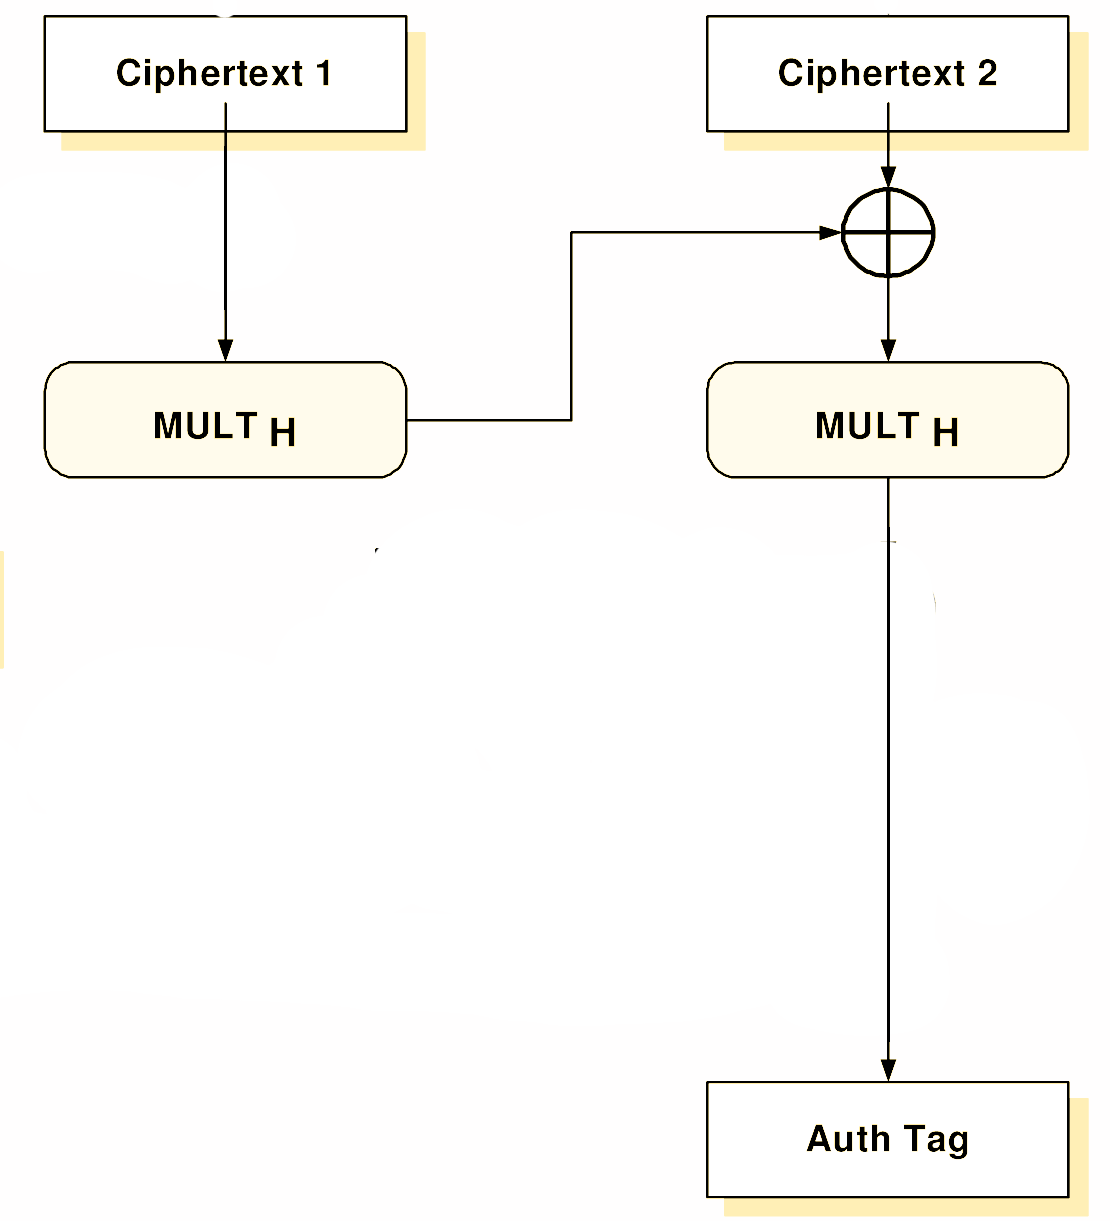
\includegraphics[width=0.4\textwidth]{auth1}
  \caption{authentification du message chiffré}
  \label{auth1}
\end{figure}

%~\\

Mais on ne veut pas seulement vérifier l'intégrité du message mais également du vecteur d'initialisation IV. Pour cela on réalise un \og et\fg{} logique entre la longueur de message et la longueur de l'IV
puis un XOR avec le tag précédent. Enfin, on effectue un bloc de Multiplication dans l'espace de Galois toujours avec la clef H comme on peut le voir sur l'image \ref{auth2}.

\begin{figure}[!h]
  \centering
  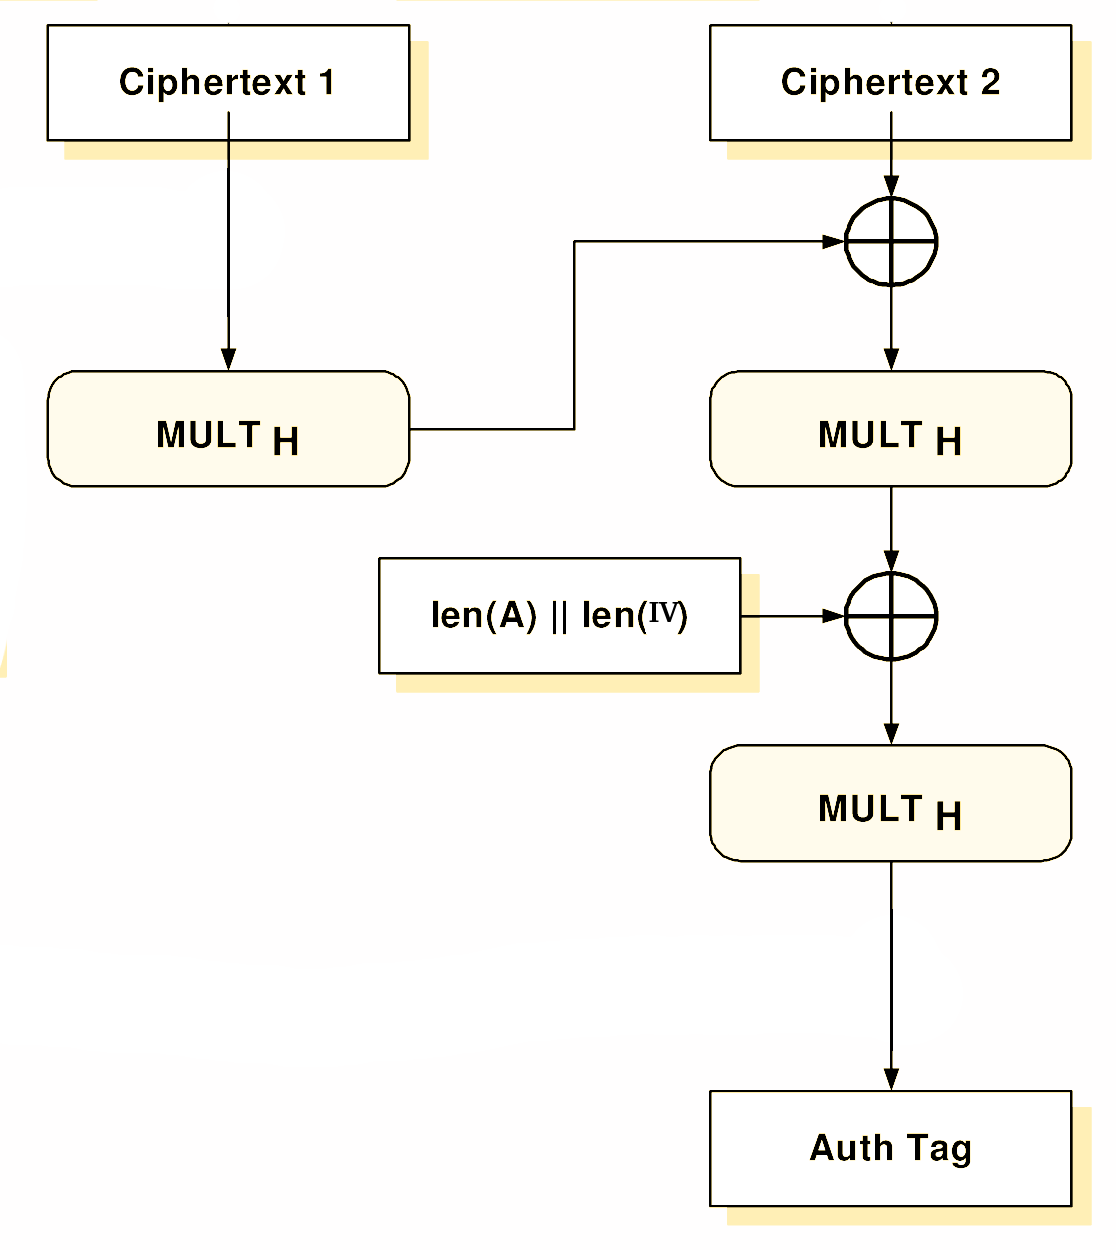
\includegraphics[width=0.4\textwidth]{auth2}
  \caption{authentification de la longueur du message et de IV}
  \label{auth2}
\end{figure}

%~\\

Ensuite, lors d'une communication entre Alice et Bob il y a des protocoles qui sont utilisés pour communiquer comme TCP/IP. Il y a donc des données qui vont entourer le message comme l'adresse IP qui permettent d'authentifier l'émetteur. Pour être certain que le message n'a pas été intercepté, on va intégrer ces données à notre tag d'intégrité et ainsi assurer l'authenticité du message. 
Au début de l'algorithme, on fait passer ces données dans un bloc de multiplication puis on réalise un XOR avec le premier bloc chiffré comme on peut le voir sur l'image \ref{auth3}.

\begin{figure}[!h]
  \centering
  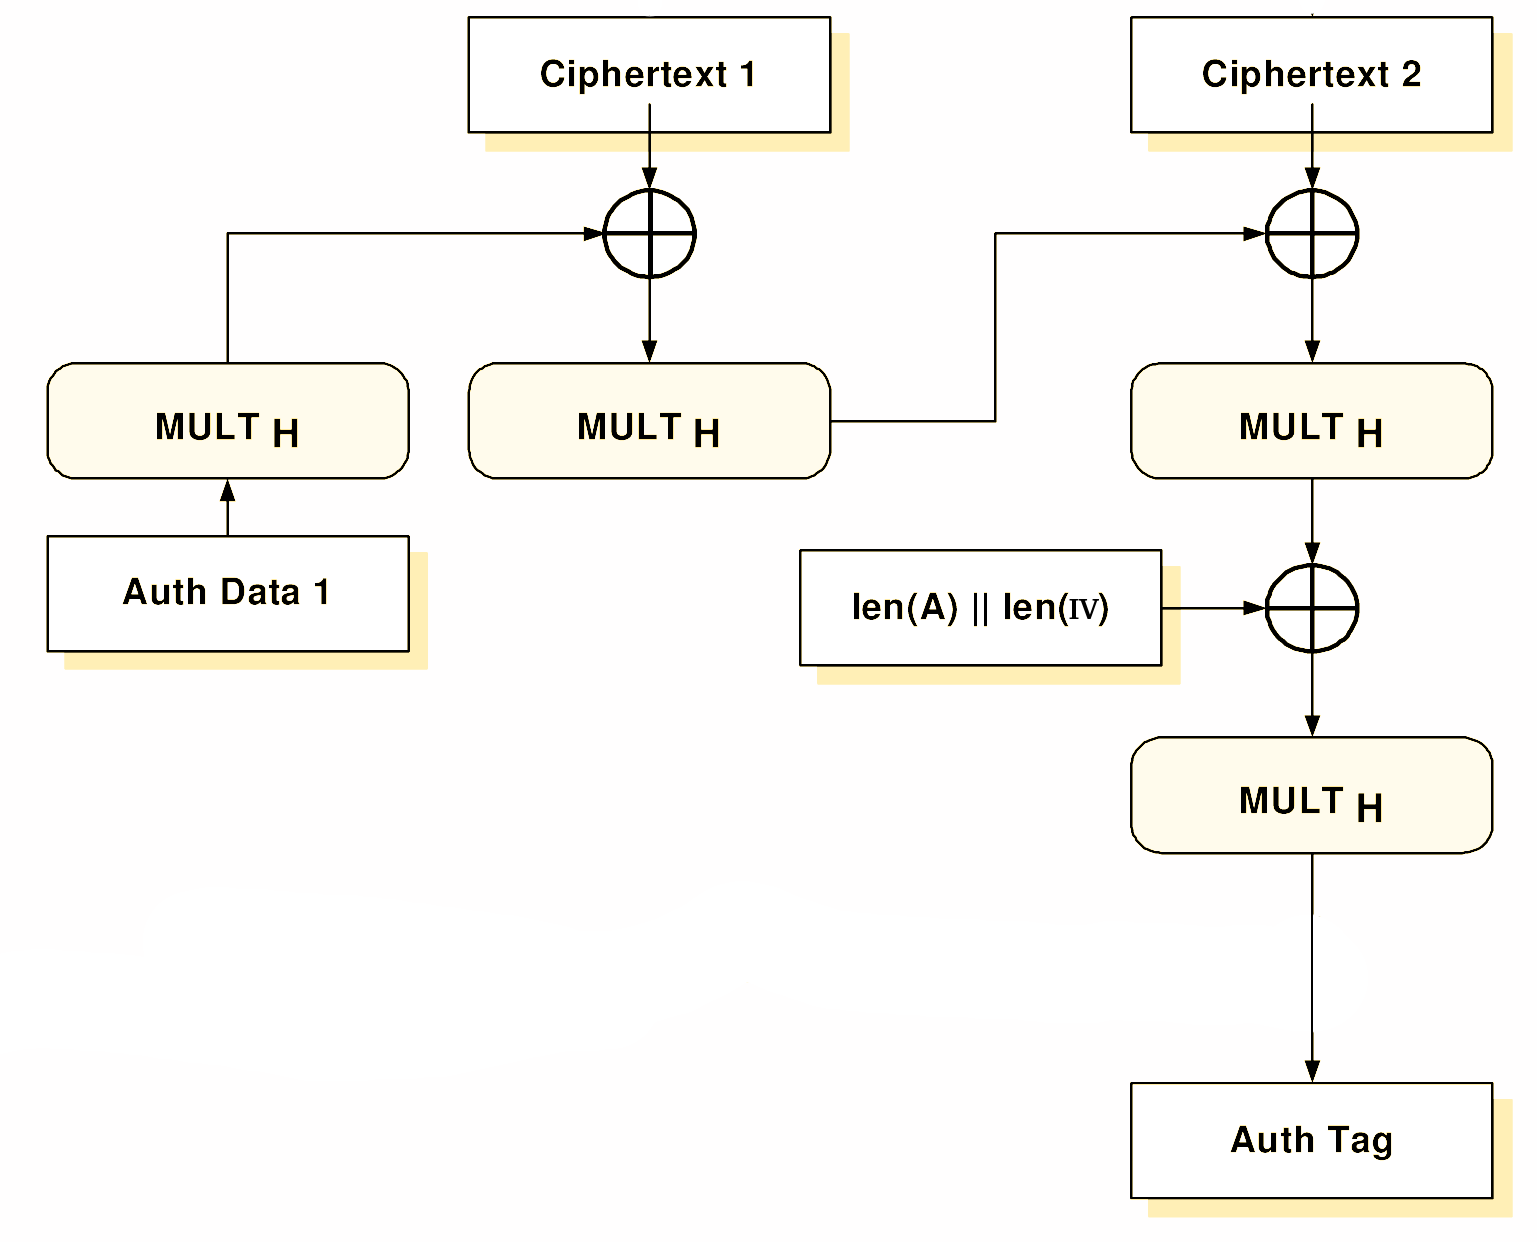
\includegraphics[width=0.5\textwidth]{auth3}
  \caption{authentification de data supplémentaire}
  \label{auth3}
\end{figure}



Nous avons donc l'intégrité et l'authenticité du message, de la longueur de IV, de la longueur du message, et des données périphériques au message, mais pour terminer l'intégrité des données on va ajouter à ceci l'IV et la clef K. %pour être certain que personne n'a touché a notre vecteur d'initialisation ainsi que
Pour cela nous chiffrons l'IV avec un compteur à 0 avec la clef K à travers l'algorithme AES. Puis nous réalisons un XOR avec le tag précédent comme on peut le voir sur l'image \ref{auth4}.

On obtient donc un tag qui permet de vérifier l'intégrité de tous les paramètres du message et l'authenticité de l'émetteur.

\begin{figure}[!h]
  \centering
  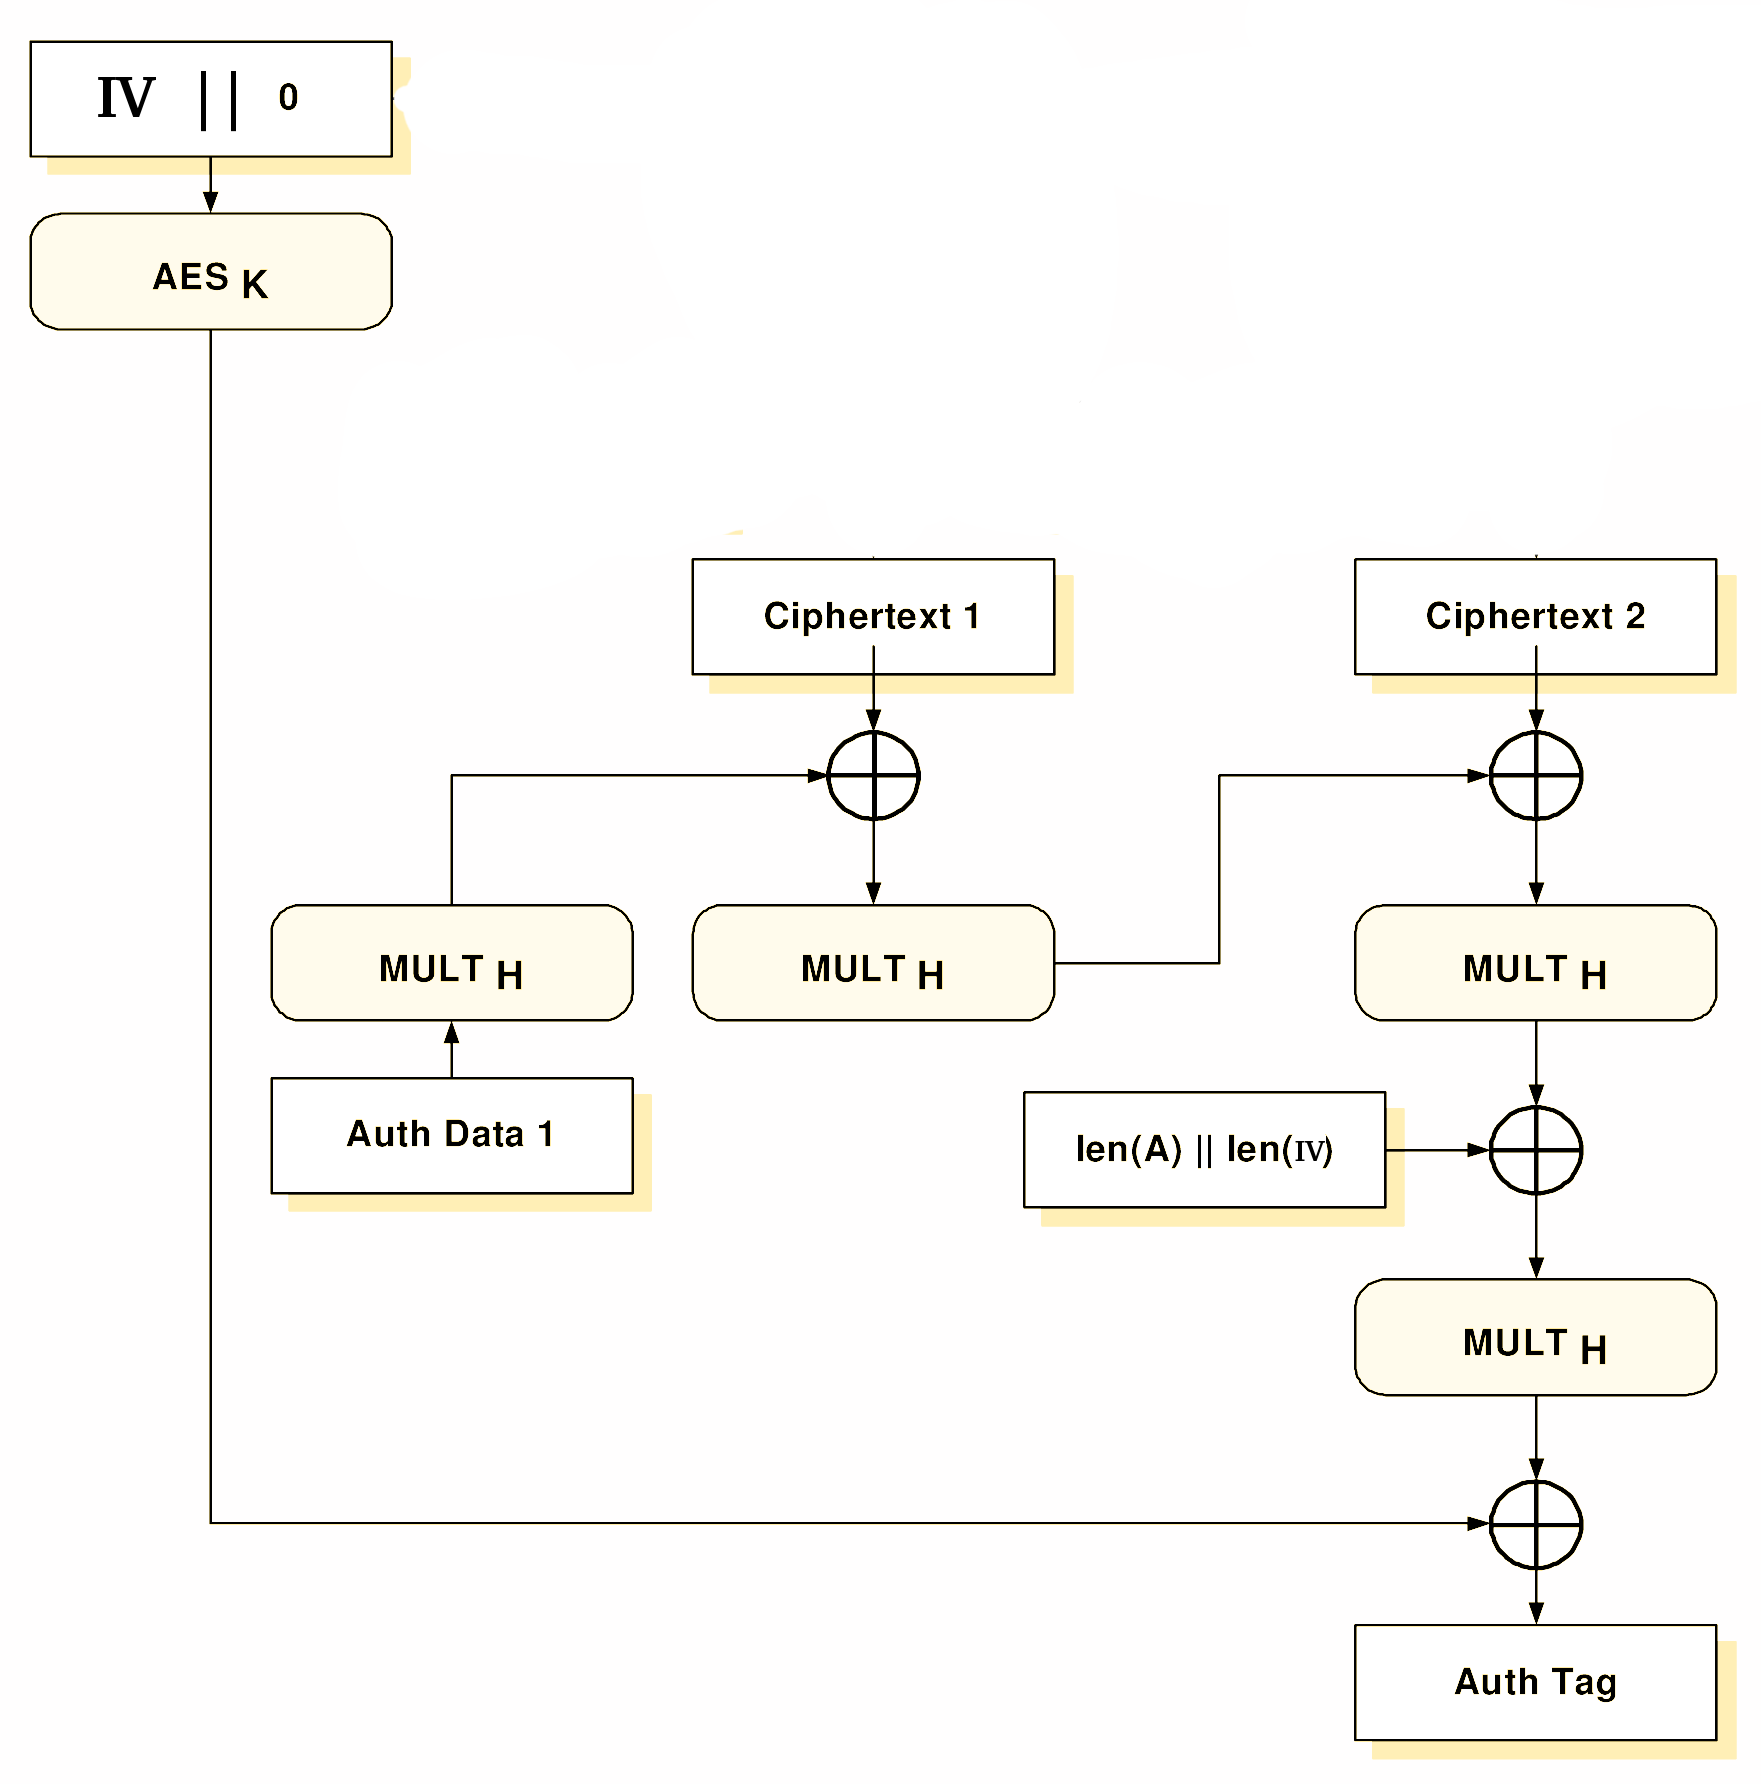
\includegraphics[width=0.5\textwidth]{auth4}
  \caption{authentification de la clef K}
  \label{auth4}
\end{figure}


Le fonctionnement global de \aes est résumé sur l'image \ref{Fonctionnement de GCM}.


\begin{figure}[!h]
  \centering
  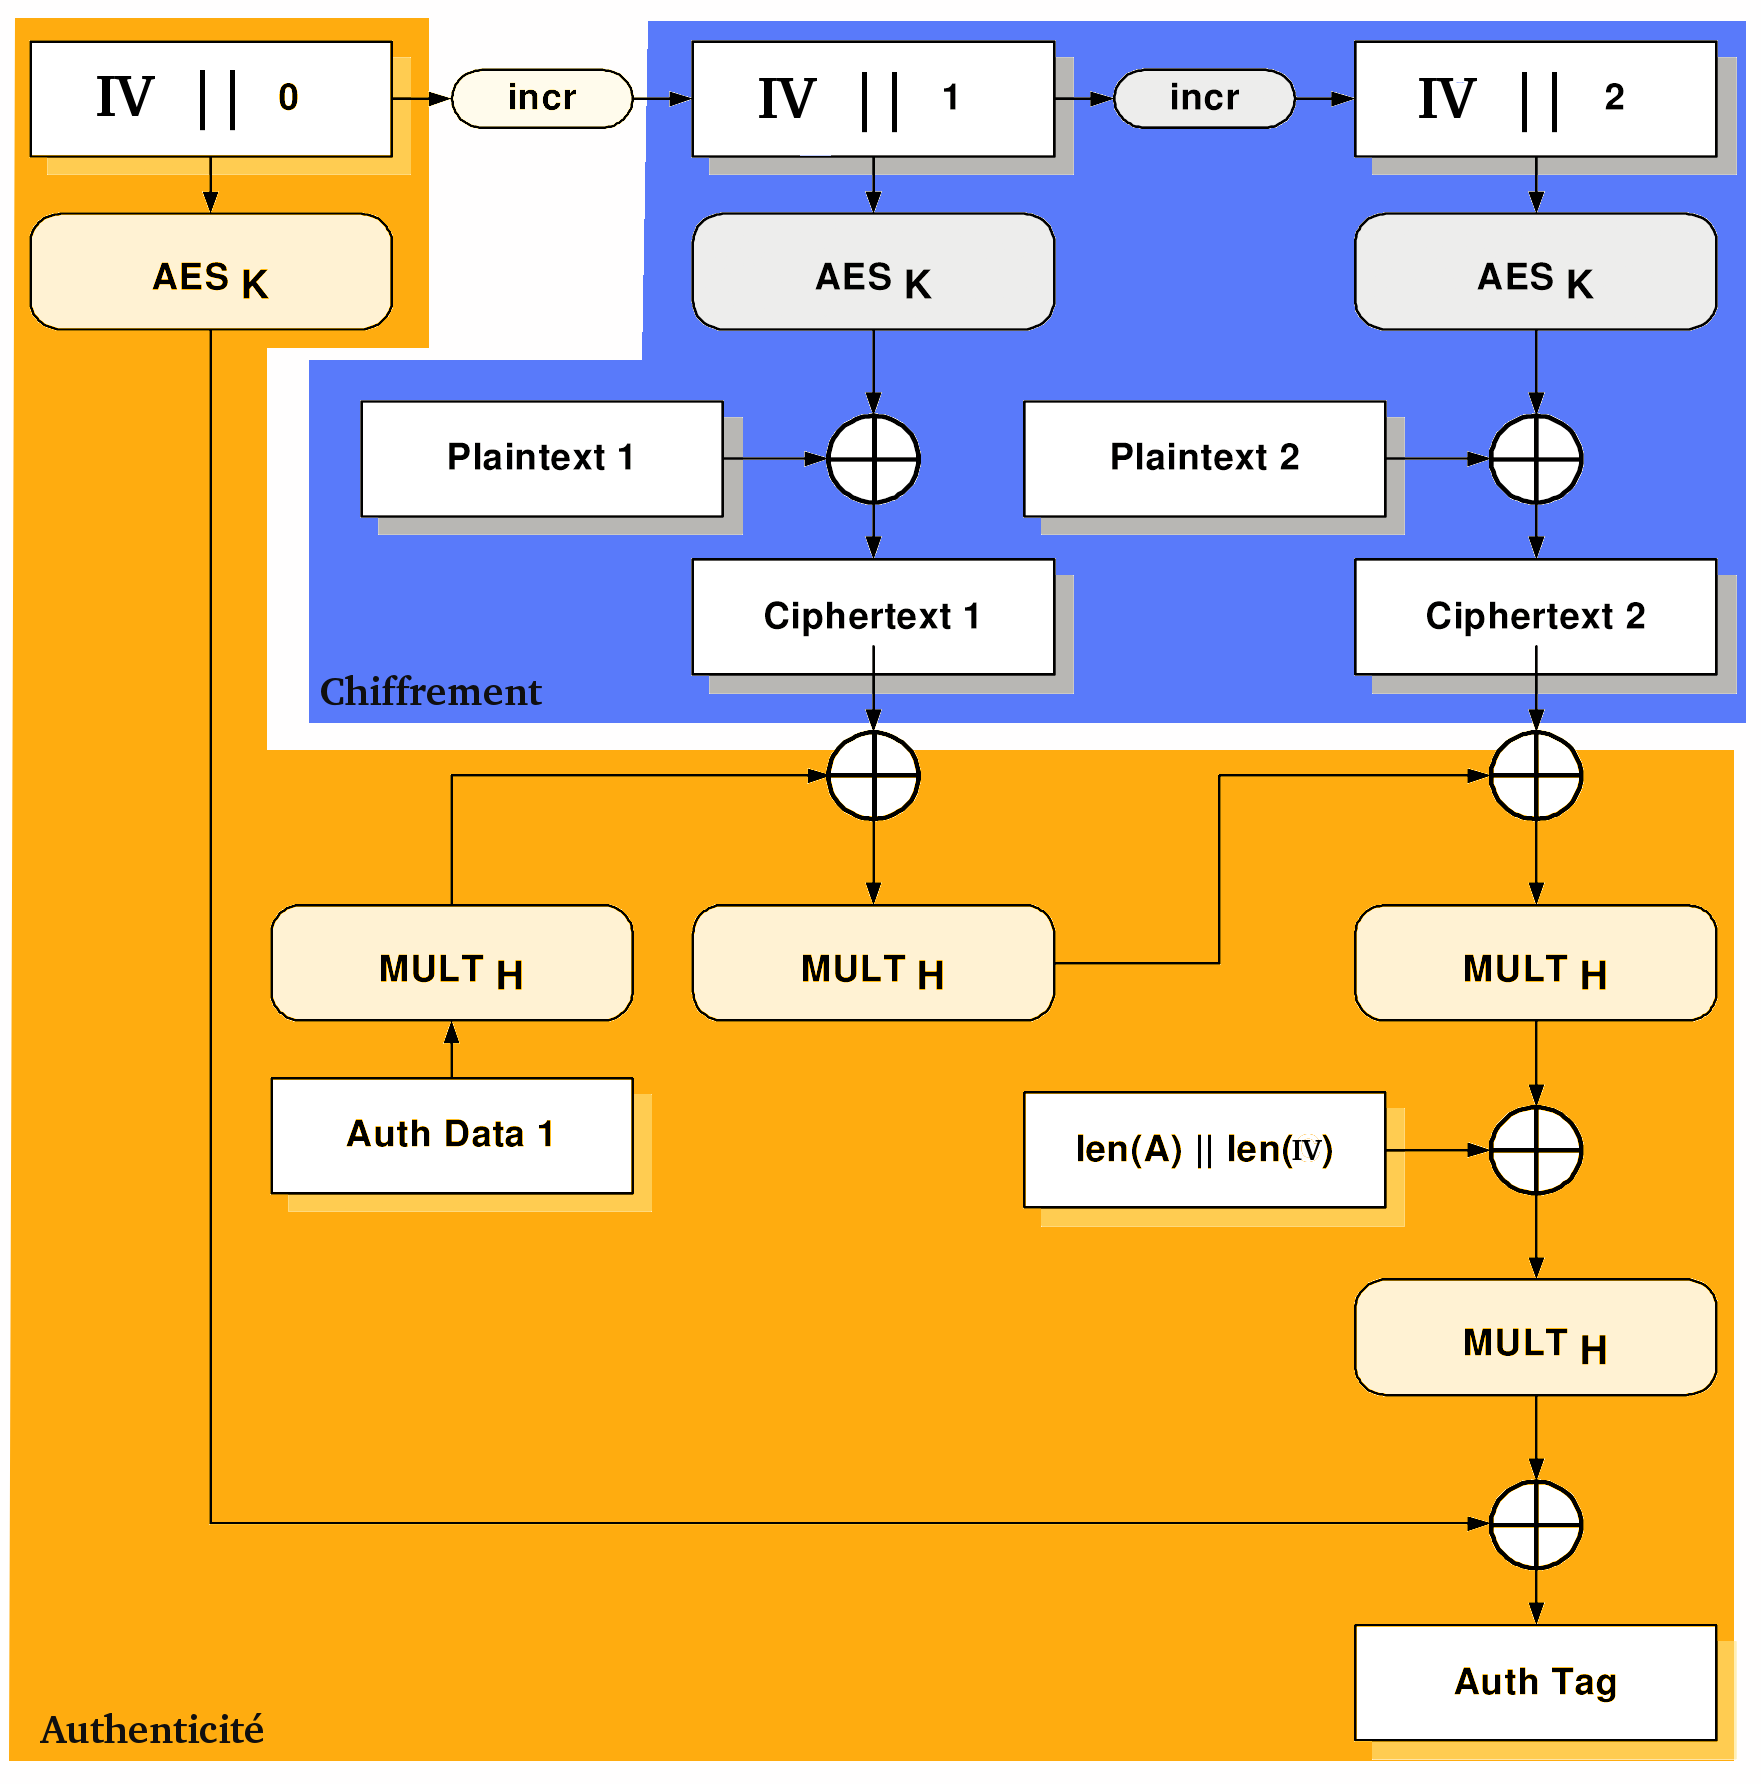
\includegraphics[width=0.8\textwidth]{fonctionnement3}
  \caption{Fonctionnement de GCM}
  \label{Fonctionnement de GCM}
\end{figure}


\subsection{Déchiffrement}

A COMPLETER


\section{GMAC}

GMAC est un cas particulier de GCM où aucun texte brut n'est présenté.




%%% Local Variables: 
%%% mode: latex
%%% TeX-master: "rapport_de_base"
%%% End: 
